\documentclass{report}
\usepackage{ifxetex}
\usepackage[svgnames]{xcolor}
\ifxetex{%
  \usepackage{fontspec}
  \setmainfont{Linux Libertine O} % or any font on your system
  \newfontfamily\quotefont[Ligatures=TeX]{Linux Libertine O} % or any font on your system
\else
  \usepackage[utf8]{inputenc}
  \usepackage[T1]{fontenc}
  \usepackage{libertine} % or any other font package (or none)
  \newcommand*\quotefont{\fontfamily{fxl}} % selects Libertine for quote font
\fi
\usepackage{tikz}
\usepackage{framed}
\usepackage{hyperref}

% Make commands for the quotes
\newcommand*{\openquote}{\tikz[remember picture,overlay,xshift=-15pt,yshift=-10pt]
     \node (OQ) {\quotefont\fontsize{30}{30}\selectfont``};\kern0pt}
\newcommand*{\closequote}{\tikz[remember picture,overlay,xshift=15pt,yshift=10pt]
     \node (CQ) {\quotefont\fontsize{30}{30}\selectfont''};}
% select a colour for the shading
\definecolor{shadecolor}{named}{Azure}
% wrap everything in its own environment
\newenvironment{shadequote}%
{\begin{snugshade}\begin{quote}\openquote}
{\hfill\closequote\end{quote}\end{snugshade}}

\begin{document}
\section*{Progress since the poster day}
After my presentation at the poster day on Feburary 6th Dr Weir had recommended I look in to the concept of "Ngram Generation" in order to aid with issues I had mentioned with the multi-term frequency calculations. After a little background reading on the subject i had set to work on generating the possible Ngrams for the dataset (or black list). The biggest issue that occurred during the development of these Ngrams has been described below.
\begin{description}
\item[Concurrent Access Exceptions]
In order to generate the algorithms in a relativley memory efficient way I constantly read from file, modify the line and then write it back. In a vain attempt at speeding up the process I decided to use a multi-threaded approach to this aspect of the application, which caused access violations as each thread began to access the file at the same time. In order to fix this issue, I abanonded the multi-threaded approach and made a slightly more elegant single threaded approach duplicating the black list stored in memory and modifying the duplicate.
\end{description}


\section*{Addressing the second assessors comments}
Below is a list of the recommendations made by my second assessor and how i have addressed them.
\begin{shadequote}
At this stage I would recommend the production of a draft background and related works chapter to get this out of the way and also to inform/measure future development.
\end{shadequote}
As suggested i have begun to draft a report on specific areas of background reading, as well as the use of Mendeley Desktop to keep track of which papers are being used as reference.
\\
\begin{shadequote}
A number of design and implementation decisions still need to be pinned down and it’s important that this is done without undue delay since the final product will need to demonstrate some novelty and innovation.
\end{shadequote}
In order to address design issues i have written the package as a toolkit (S.T.E.L.A ~ The Strathclyde Toolkit for Explicit Language Analysis) allowing for use with any other applications. This also allows a speedy development of a front end in terms of the project.
\\
\begin{shadequote}
Likewise, a good evaluation strategy will need to be adopted and results from this analysed to produce a valid comparison with other, related, systems. Ethics approval needs also to be sorted out ASAP given the nature of the project.
\end{shadequote}
In terms of evaluation I have made good progress towards the preparation for tests. I have sent several draft applications for ethics approval to Dr Weir and I aim to carry out the experiment by the week ending the 8'th of March, leaving me a little over two weeks to write the evaluation report and compare the results. Also following the seminar presented by Dr Dunlop, I have created an excel spreadsheet for gathering data from the experiments a copy of which can be found at \url{https://github.com/chris-forbes-1/measuring_content/blob/Experimental/Experiment Calculations.xlsx}
\\
\section*{Next steps}
As discussed at the poster day, the next step will be to add weights to the blacklist words. I am also aiming to impliment a modified version of the sentiment analysis described in 'Sentiment analysis: Capturing favorability using natural language processing by Tetsuya Nasukawa and Jeonghee Yi'.

\section*{Alterations to project plan}
Very few alterations have been made to the project plan. I have added a separate step into the project plan to account for the inclusion of sentiment analysis in to the toolkit.
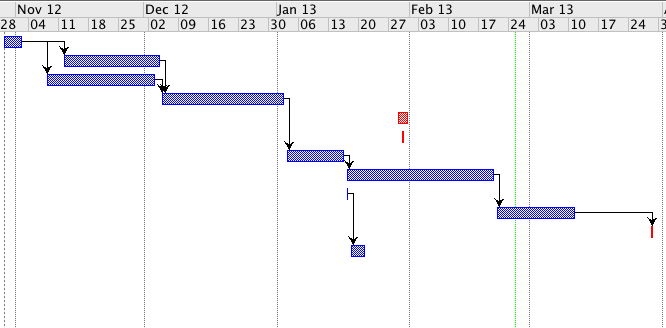
\includegraphics[scale=0.5]{ProjPlan.png}
\end{document}
